\documentclass{beamer}
\usepackage[utf8]{inputenc}
\usepackage{tikz}
\usepackage{graphicx}
\usetheme{Warsaw}

\title{Les architectures SIMD}
\author{Victor Hiairrassary}
\institute{Polytech' Montpellier}
\date{28 mars 2012}

% On enlève la barre de navigation
\setbeamertemplate{navigation symbols}{}

% TODO: Afficher le plan!


\begin{document}

% On diminue la police
\small 


\begin{frame}
    \titlepage
\end{frame}


\begin{frame}{Introduction}
    \begin{block}{Définition}
    SIMD, pour Single Instruction on Multiple Data, correspond à une instruction
    processeur qui va s'éxécuter simultanément sur un lot particulier de données.
    \end{block}

    \begin{figure}
    \begin{center}
        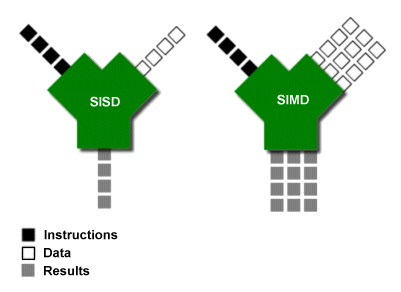
\includegraphics[scale=0.3]{simd.png}
    \end{center}
     \caption{Schéma simplifiée d'une architecture SIMD}
    \end{figure}

    \begin{block}{}
    Il existe plusieurs jeux d'instructions SIMD, certains propres à une époque, 
    d'autres à une architecture.
    \end{block}
\end{frame}


\begin{frame}{Historique}
    \begin{block}{Processeurs x86}
    Les premières instructions SIMD s'appellent MMX et sont apparues en 1997
    grâce à Intel. Jugées peu performantes, AMD sort 3DNow!
\newline \newline
    En réponse, Intel invente les intructions SSE pour processeurs x86 qui vont 
    littéralement envahir le marché. Ce sont des opérations sur des registres 
    128 bits. Elles subirent plusieurs extensions (à ce jour 4.2). 
\newline \newline
    Intel se concentre désormais sur ses dernières instructions SIMD : AVX.
    Celles-ci opèrent sur des registres 256 bits.
    \end{block}

    \begin{block}{Autres}
    Chez les concurrents on trouve :
        \begin{itemize}
        \item ARM : Neon
        \item SPARC : VIS et VIS2
        \item MIPS : MDMX et MIPS-3D
        \end{itemize}
    \end{block}
\end{frame}


\begin{frame}{Applications}
    \begin{block}{Alignement}
    Le modèle SIMD convient particulièrement bien aux traitements dont la 
    structure est très régulière.
\newline \newline
    Quelques domaines :
        \begin{itemize}
        \item Calcul matriciel
        \item Cryptographie (manipulation de grands nombres)
        \item Codecs audio et vidéo
        \item Compression
        \end{itemize}
    \end{block}

    \begin{block}{Remarque}
    Les instructions SIMD ne sont pas réserveés aux CPU! On en trouve aussi
    beaucoup dans les GPU.
    \end{block}
\end{frame}


\begin{frame}{Registres MMX}
    \begin{block}{Alignement}
    Afin de pouvoir utiliser des instructions SSE, il faut au préalable avoir
    aligné sur 16 bits la mémoire allouée pour les données! Sinon c'est une 
    erreur assurée.
\newline \newline
    La figure ci-dessous montre la pile de registres du jeux d'instructions MMX,
    utilisée par les instructions SSE. Ils sont chacun sur 128 bits.
    \end{block}

    \begin{figure}[!t]
    \begin{center}
        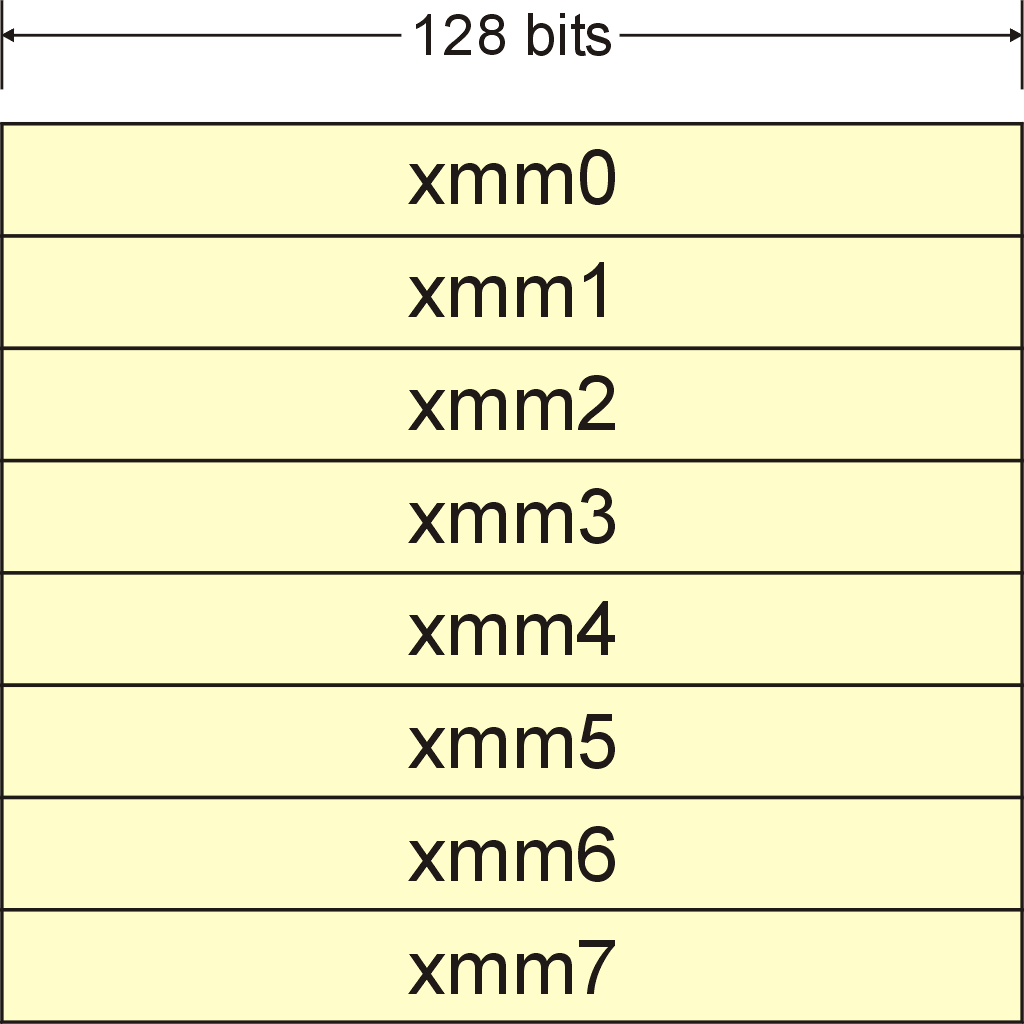
\includegraphics[scale=0.13]{XMM_registers.png}
    \end{center}
     \caption{Schéma des registres MMX}
    \end{figure}
\end{frame}


\begin{frame}[fragile]{Exemple}
    \begin{block}{Exemple}
    Ci-dessous un exemple concret d'utilisation des instructions SSE, extrait de
    la documentagtion officielle de Intel. C'est l'instruction addps qui ajoute 
    deux registres de 128 bits entre eux. Le tout en seulement 2 ou 3 cycles!!
    \end{block}
\tiny
    \begin{verbatim}
ADDPS		Add Parallel Scalars

Opcode      Cycles  Instruction
0F 58       2 (3)   ADDPS xmm reg,xmm reg/mem128

ADDPS op1, op2

op1 contains 4 single precision 32-bit floating point values
op2 contains 4 single precision 32-bit floating point values

	op1[0] = op1[0] + op2[0]
	op1[1] = op1[1] + op2[1]
	op1[2] = op1[2] + op2[2]
	op1[3] = op1[3] + op2[3]
    \end{verbatim}
\small

\end{frame}


\begin{frame}{Avantages}
    \begin{block}{Avantages}
        \begin{itemize}
        \item Certains compilateurs peuvent automatiquement utiliser ces instructions (msvc, gcc, icc, etc).
        \item De nombreuses APIs pour les utiliser.    
        \item Des performances fortement accrues (le diagramme ci-dessous correspond aux 
        résultats du benchmarck sur le blog supercomputing, cf. bibliographie).
        \end{itemize}

        \tiny

        \begin{center}
        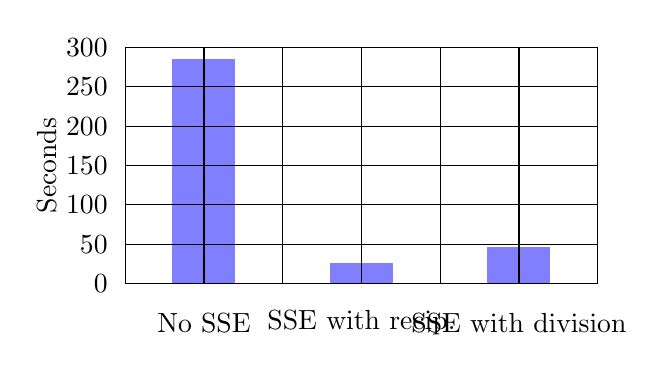
\begin{tikzpicture}[yscale=0.5]
            \draw[line width=8mm, color=blue!50] plot[ycomb] coordinates { (1, 5.7) (3, 0.52) (5, 0.93) };
            \draw (0,0) grid (6,6);
            \draw (1,-1) node{No SSE};
            \draw (3,-1) node{SSE with recip.};
            \draw (5,-1) node{SSE with division};
            \draw (-1,3) node[rotate=90]{Seconds};
            \foreach \y in {0,50,...,300} \draw (-0.1, \y/50)node[left]{\y};
        \end{tikzpicture}
        \end{center}

        \small

    \end{block}
\end{frame}


\begin{frame}{Inconvénients}
    \begin{block}{Inconvénients}
        \begin{itemize}
        \item Le programme dépend du processeur hôte.
        \item Certains algorithmes ne peuvent pas utiliser les instructions SIMD de
        par leur nature, comme tout ce qui touche au parsing par exemple.
        \item Nécessite une connaissance bas niveau.
        \item Les compilateurs ne savent pas toujours le faire tout seul. La 
        "vectorisation" est un sujet de recherche.
        \end{itemize}
    \end{block}
\end{frame}


\begin{frame}{Conclusion}
    \begin{block}{Conclusion}
    On retiendra donc des instructions SIMD qu'elles permettent grandement 
    d'accélérer certains calculs.
\newline \newline
    Il existe également des outils et APIs permettant de s'abstraire de cela, 
    tout en utilisant la puissance du SIMD en interne, comme boost.simd en C++.
    \end{block}
\end{frame}


\begin{frame}{Bibliographie}
    \begin{block}{Liens}
        \begin{itemize}
        \item Documentation SSE Intel : \url{http://www.intel80386.com/simd/mmx2-doc.html}
        \item The supercomputing blog : \url{http://supercomputingblog.com/optimization/getting-started-with-sse-programming/}
        \item Wikipédia : \url{http://en.wikipedia.org/wiki/SIMD}
		\item boost.simd : \url{https://github.com/boostcon/2011_presentations/raw/master/thu/simd.pdf}
        \end{itemize}
    \end{block}
\end{frame}


\end{document}
